%%%%%%%%%%%%%%%%%%%%%%%%%%%%%%%%%%%%%%%%%%%%%%%
%%% Template for lab reports used at BIT modified from STIMA
%%% Author: Charlie Li
%%%%%%%%%%%%%%%%%%%%%%%%%%%%%%%%%%%%%%%%%%%%%%%

%%%%%%%%%%%%%%%%%%%%%%%%%%%%%% Sets the document class for the document
% Openany is added to remove the book style of starting every new chapter on an odd page (not needed for reports)
\documentclass[12pt,openany,a4paper]{book}
%%%%%%%%%%%%%%%%%%%%%%%%%%%%%% Loading packages that alter the style
\usepackage[]{graphicx}
\usepackage[]{color}
\usepackage{alltt}
\usepackage[T1]{fontenc}
\usepackage[utf8]{inputenc}
\usepackage{polski}
% \usepackage[polish]{babel}
% Math
\usepackage{amsmath}
\usepackage{amssymb}
\usepackage{physics}
% Fonts
\renewcommand{\rmdefault}{ptm}
\renewcommand{\sfdefault}{phv}


\setcounter{secnumdepth}{3}
\setcounter{tocdepth}{3}
\setlength{\parskip}{\smallskipamount}
\setlength{\parindent}{12pt}
\usepackage{indentfirst}

% Set page margins
\usepackage[top=50pt,bottom=60pt,left=78pt,right=78pt]{geometry}
\usepackage{subcaption}
% Package used for placeholder text
\usepackage{booktabs}
\usepackage{multirow}
% Prevents LaTeX from filling out a page to the bottom
\raggedbottom{}

% Adding both languages
% \usepackage[english]{babel}

% All page numbers positioned at the bottom of the page
\usepackage{fancyhdr}
\fancyhf{} % clear all header and footers
\fancyfoot[C]{\thepage}
%\fancyhead[L]{{\selectfont \leftmark}}
\renewcommand{\headrulewidth}{0pt} % remove the header rule
\pagestyle{fancy}

% Changes the style of chapter headings
\usepackage{titlesec}
\titleformat{\chapter}
{\normalfont\LARGE\bfseries}{\thechapter.}{1em}{}
% Change distance between chapter header and text
\titlespacing{\chapter}{0pt}{40pt}{2\baselineskip}

% Adds table captions above the table per default
\usepackage{float}
\floatstyle{plaintop}
\restylefloat{table}

% Adds space between caption and table
\usepackage[tableposition=top]{caption}

% add cc license
% \usepackage[
% type={CC},
% modifier={by-nc-sa},
% version={4.0},
% ]{doclicense}

% Adds hyperlinks to references and ToC
\usepackage{hyperref}
% \usepackage[backref=page]{hyperref} % hyperlinks
% \renewcommand*{\backref}[1]{}
% \renewcommand*{\backrefalt}[4]{{\footnotesize [%
% 		\ifcase #1 Not cited.%
% 		\or Cited on page~#2%
% 		\else Cited on pages #2%
% 		\fi%
% 		]}}
\usepackage[capitalise]{cleveref}

% Uncomment the line below this block to set all hyperlink color to black
\hypersetup{
	colorlinks,
	linkcolor={blue},
	citecolor={green!90!black},
	urlcolor={red!70!black}
}
%\hypersetup{hidelinks,linkcolor = black} % Changes the link color to black and hides the hideous red border that usually is created

% Set specific color for hyperref
\usepackage{xcolor}


% tcolorbox; Notice! add "-shell-escape" to the compile command
\usepackage{tcolorbox}

% If multiple images are to be added, a folder (path) with all the images can be added here 
% \graphicspath{ {Figures/} }

% Separates the first part of the report/thesis in Roman numerals
\frontmatter
\patchcmd{\chapter}{\thispagestyle{plain}}{\thispagestyle{fancy}}{}{}{}
% Uncomment to stop the new chapter start at a new page
\usepackage{etoolbox}
\makeatletter
\patchcmd{\chapter}{\if@openright\cleardoublepage\else\clearpage\fi}{}{}{}
\patchcmd{\section}{\if@openright\cleardoublepage\else\clearpage\fi}{}{}{}
\makeatother


\usepackage{bpchem}
\usepackage{epstopdf}
\usepackage[
    backend=biber,
	% babel = other,
    style=numeric,
	sorting=none
  ]{biblatex}
\addbibresource{C:/texlive/Bibtex/AlGaAsSb.bib}
\usepackage{siunitx}
% \addbibresource{ref.bib}
%%%%%%%%%%%%%%%%%%%%%%%%%%%%%% Starts the document
\begin{document}
	

	
	%%%%% Adds the title page
	\begin{titlepage}
		\clearpage\thispagestyle{empty}
		\centering
		\vspace{1cm}
		
		% Titles
		% Information about the University
		{\
			\textsc{Projektowanie Struktur Półprzewodnikowych}
		}
		\vspace{2.5cm}
		
		\rule{\linewidth}{2mm} \\[0.8cm]
		{ \LARGE \sc Sprawozdanie}\\[0.55cm]
		\rule{\linewidth}{0.6mm} \\[3.4cm]
		
		\hspace{2cm}
		\begin{tabular}{l p{5cm}}
			\textbf{Imię} & Jakub Pawłowski \\[10pt]
			\textbf{Numer albumu} & \texttt{250193} \\[10pt]
			\textbf{Kierunek} & \texttt{Inżynieria Kwantowa} \\[10pt]
			\textbf{Rok/Semestr} & Semestr letni 2020/2021 \\[10pt]
			\textbf{Materiał} & \BPChem{AlGaAsSb} \\[10pt]
			\textbf{Data} & \today \\            
		\end{tabular}
		
		
		\vfill
		% \centering
\includegraphics{Figures/pwr.eps}
		\centering 
\includegraphics[width = \linewidth]{Figures/pwr.png}
		\vspace{0.5cm}
		
		
		
		
		\pagebreak
		
	\end{titlepage}
	%% Uncomment for title page print two pages per sheet
	%\shipout\null
	
	% Comment the following two lines to remove abstract 
	% \chapter*{\makebox[\linewidth]{Abstract}}
	% \addcontentsline{toc}{chapter}{Abstract}
	% This is a template for Projects/Report/Proposals at BIT. ~\lipsum[5]
	
	% \vspace{0.5cm}
	% \noindent\textbf{Keywords}: 
	% \LaTeX, BIT
	% \clearpage
	
	% Adds a table of contents keep the link black
	\let\cleardoublepage\clearpage
	{\hypersetup{linkcolor=black}
		% or \hypersetup{linkcolor=black}, if the colorlinks=true option of hyperref is used
		\tableofcontents{}
	}
	
	%%%%%%%%%%%%%%%%%%%%%%%%%%%%%%%%%%%%%%%%%%%%%%%%%%%%%%%%%%%%%%%%%%%%%%%%%%%%%%%%%%%%%%%%%%%%
	%%%%%%%%%%%%%%%%%%%%%%%%%%%%%%%%%%%%%%%%%%%%%%%%%%%%%%%%%%%%%%%%%%%%%%%%%%%%%%%%%%%%%%%%%%%%
	%%%%% Text body starts here!
	\mainmatter{}
	
	
	\chapter{Opis systemu materiałowego}\label{chapt:opis}
	
	Badanym materiałem jest czteroskładnikowy stop \BPChem{AlGaAsSb}. Znajduję on zastosowanie m.in. w budowie
	laserów na heterostrukturach~\autocite{Morosini1993}, kaskadowych ogniw słonecznych~\autocite{Timmons1981} oraz
	w charakterze szerokopasmowego źródła światła wysokiej mocy, na zakresie spektralnym \SI{2.2}{\micro\metre} do \SI{2.5}{\micro\metre},
	opartego na studni kwantowej~\autocite{Wootten2014}.\\

	Składa się on z 4 materiałów binarnych, związków III-V tj.:
	\begin{itemize}
		\item \BPChem{AlAs}
		\item \BPChem{AlSb}
		\item \BPChem{GaAs}
		\item \BPChem{GaSb}
	\end{itemize} 
	Informacje o materiałach binarnych posłużą nam do wyznaczenia podstawowych parametrów materiałowych.
	Związki III-V w rozpatrywanym stopie czteroskładnikowym mieszają się, tworząc stopy trójskładnikowe.
	Są to:
	\begin{itemize}
		\item \BPChem{AlGaAs}
		\item \BPChem{AlGaSb}
		\item \BPChem{AlAsSb}
		\item \BPChem{GaAsSb}
	\end{itemize}
	
	\section{Zastosowania materiałów binarnych}
	\BPChem{AlAs}, \BPChem{GaAs}, \BPChem{AlSb} oraz \BPChem{GaSb} tworzą kryształy o strukturze blendy cynkowej (stałe sieciowe odpowiednio \SI{5.6611}{\angstrom}, \SI{5.6533}{\angstrom}, \SI{6.1355}{\angstrom} oraz \SI{6.0959}{\angstrom}) i grupie przestrzennej
	\(F\overline{4}3m\). Parametry materiałowe opisujące te związki można znaleźć w~\textcite{Adachi1985,Vurgaftman2001,Adachi1989,Adachi2017}.


	\BPChem{AlSb} jest półprzewodnikiem grupy III-V o przerwie energetycznej \SI{1.6}{\electronvolt}. Ze względu na możliwość
	hodowli dużych, pojedynczych kryształów o ruchliwości elektronów do \SI{350}{\centi\metre^2\per\volt\second} materiał ten jest
	wykorzystywany jako detektor fotonów~\autocite{Seeger1991}.

	\BPChem{GaAs} jest półprzewodnikiem grupy III-V o przerwie energetycznej \SI{1.441}{\electronvolt}. Jest to jeden
	z najbardziej popularnych półprzewodników. Stosowany zarówno w charakterze emitera promieniowania np. diody LED świecące
	w bliskiej podczerwieni~\autocite{Hall1962} oraz absorbera, umożliwiając konstrukcję bardzo wydajnych ogniw słonecznych,
	zbliżających się do limitu Shockleya–Queissera~\autocite{Wang2013}.

	\BPChem{GaSb} jest półprzewodnikiem grupy III-V o wąskiej przerwie energetycznej \SI{0.67}{\electronvolt}~\autocite{Dubey2006}.
	Materiał ten ma duży potencjał do zastosowań elektro-optycznych w zakresie bliskiej podczerwieni. Homozłącza oparte na \BPChem{GaSb}
	są dobrym kandydatem na szybkie fotodiody lawinowe o niskim szumie~\autocite{Milnes1993}. Ze względu na stałą sieciową zgodną z różnymi
	trój- i czteroskładnikowymi stopami III-V, pokrywającymi szeroki zakres spektralny od \SI{0.8}{\micro \metre} do \SI{4.3}{\micro \metre}
	znajduje on zastosowanie jako substrat do tworzenia źródeł i detektorów~\autocite{Dutta1997}. Wykorzystywany jest również do budowy diód
laserowych oraz fotodetektorów o wysokiej wydajności kwantowej~\autocite{Hildebrand1980,Hildebrand1981}.

\BPChem{AlAs} jest półprzewodnikiem grupy III-V o skośnej przerwie wzbronionej \SI{2.16}{\electronvolt}~\autocite{Bouarissa2009}.
	Materiał ten znajduje zastosowanie jako emiter, np. do budowy stosowanych w spektroskopii kwantowych laserów kaskadowych operujących na zakresie
	spektralnym odpowiadającym częstością \SI{3.4}{\tera\hertz} do \SI{5}{\tera\hertz} co odpowiada bliskiej podczerwieni~\autocite{Schrottke2016}.


\section{Zastosowania stopów trójskładnikowych}
\BPChem{Al\_{x}Ga\_{1-x}As} jest materiałem półprzewodnikowym zbliżonym pod względem stałej sieciowej do \BPChem{GaAs},
jednak o większej przerwie wzbronionej, która zmienia się między \SI{1.42}{\electronvolt} a \SI{2.16}{\electronvolt}.
Dla \(x < 0.4\) przerwa fundamentalna jest prosta. Znajduje on zastosowanie do budowy wydajnych fotodetektorów
opartych na studiach kwantowych i pracujących w zakresie podczerwieni~\autocite{Kock1992a}. W tym materiale zaobserwowane
zostały również nieliniowe efekty optyczne~\autocite{Aitchison1997}.

\BPChem{Al\_{x}Ga\_{1-x}Sb} jest materiałem półprzewodnikowym grupy III-V. Przypomina on \BPChem{Al\_{x}Ga\_{1-x}As} tylko o niższej
przerwie wzbronionej. Znajduje on zastosowanie do budowy fotodetektorów pracujących w podczerwieni~\autocite{Law1981}, w tym do diod lawinowych~\autocite{Hildebrand1980,Hildebrand1981}.


\BPChem{AlAs\_{x}Sb\_{1-x}} jest materiałem półprzewodnikowym grupy III-V. Stosowany jest w charakterze zarówno detektora, do budowy
nisko zaszumionych diód lawinowych~\autocite{Tan2012} oraz emitera, w kwantowych laserach kaskadowych o długości fali ok. \(\lambda = \SI{3.7}{\micro\metre}\)
w temperaturze pokojowej, a więc pracujących w zakresie bliskiej podczerwieni~\autocite{Yang2006}.

\BPChem{GaAs\_{1-x}Sb\_{x}} jest materiałem półprzewodnikowym grupy III-V. Stosowany jest głównie jako
fotodetektor pracujący w bliskiej podczerwieni~\autocite{Sun2002,Li2015}. Innym interesującą aplikacją
tego materiału jest zwiększenie długości fali emitowanej z kropki kwantowej \BPChem{InAs/GaAs}, poprzez
naniesienie jego cienkiej warstwy zmniejszającej naprężenia w kropce~\autocite{Liu2005}.



Parametry nieliniowości stopów trójskładnikowych mogą zostać znalezione w \textcite{Vurgaftman2001,Linnik2000,Adachi1989,Adachi2017,Mozume2008}.



% \section{test}
	

\chapter{Opis modeli i metod}\label{chapt:methods}
\section{Schemat interpolacyjny}\label{sec:interpolation}
W celu znalezienia parametrów stopów trójskładnikowych znając parametry materiałów binarnych
	możemy posłużyć się dobrze znanym schematem interpolacyjnym~\autocite{Adachi1985}. W najprostszym, liniowym
	przybliżeniu parametr \(T\) materiału trójskładnikowego  może zostać wyznaczonych przy pomocy
	parametrów binarnych korzystając ze wzoru:
	\begin{equation}
		T_{A_x B_{1-x}C}(x) = x B_{AC} + (1-x)B_{BC} \equiv a + bx
		\label{eq:linear_interp}
	\end{equation}
	gdzie \(a = B_{BC}\) oraz \(b = B_{AC}-B_{BC}\)
	W praktyce, niektóre parametry materiałowe znacznie odbiegają od
	relacji~\eqref{eq:linear_interp} i wykazują w przybliżeniu kwadratową
	zależność od ułamka molowego \(x\)~\autocite{Adachi2017}:
	\begin{equation}
		T_{A_x B_{1-x}C}(x) = x B_{AC} + (1-x)B_{BC}  - C_{A-B}x(1-x)\equiv a + bx+cx^2
		\label{eq:quadratic}
	\end{equation} 
	gdzie \(a = B_{BC}\), \(b = B_{AC} - B_{BC}+C_{A-B}\) oraz \(c = C_{A-B}\). Parametr \(c\)
	to tzw. bowing parameter czyli parametr nieliniowości. Tym równaniem będziemy się posługiwali
	do wyznaczenia własności stopów trójskładnikowych, w przypadku liniowym podstawiając
	wartość \(0\) za parametr nieliniowości.\\

	W przypadku, gdy interesują nas własności stopu czteroskładnikowego postaci
	\BPChem{A\_{x}B\_{1-x}C\_{y}D\_{1-y}}, a znamy już własności stopów trójskładnikowych
	składających się na ten materiał możemy posłużyć się następującym związkiem~\autocite{Adachi2017}:
	\begin{align}
		Q(x,y) = & \frac{x(1-x)\left[y T_{ABC}(x) + (1-y)T_{ABD}(x)\right]}{
			x(1-x) + y(1-y)} \\
			&+ \frac{y(1-y)\left[x T_{ACD}(y) + (1-x)T_{BCD}(y)\right]}{x(1-x) + y(1-y)}
			\label{eq:quaternary} 
	\end{align}

\section{Parametry materiałów binarnych. Parametry nieliniowości.}\label{sec:binary_params}

Większość wykorzystanych parametrów materiałów binarnych oraz parametrów nieliniowości
pochodzi z pracy przeglądowej~\citetitle{Vurgaftman2001},~\textcite{Vurgaftman2001}, za wyjątkiem mas
efektywnych dziur lekkich, ciężkich oraz odpowiednich parametrów nieliniowości,
które zostały zaczerpnięte z książki~\citetitle{Adachi2009},~\textcite{Adachi2009}.
Parametry materiałów binarnych zostały przedstawione w tabeli~\ref{tab:binary}
\begin{table}[htbp]
	\centering
	\caption{Parametry materiałów binarnych~\autocite{Vurgaftman2001,Adachi2009}}
	  \begin{tabular}{ccccc}
	  \toprule
	  \toprule
	  Parametr & \BPChem{AlAs} & \BPChem{AlSb} &  \BPChem{GaSb} & \BPChem{GaAs}\\
	  \midrule
	  \(E_g^{\Gamma}\)(eV)  &3.099 &2.386 &0.812 &1.519  \\
	  VBO (eV)   & -1.33&-0.41 &-0.03 & -0.80 \\
	  \(\Delta_{\textrm{SO}}\) (eV)  &0.28 &0.676 &0.76 & 0.341 \\
	  \(a_{lc}\) (\AA) &5.6611 &6.1355 & 6.0959& 5.65325\\
	  \(m_e^{\ast}\)    &0.15 & 0.14& 0.039& 0.067 \\
	  \(m_{hh}^{\textrm{DOS}}\)  &0.81 &0.9 &0.37 & 0.55 \\
	  \(m_{lh}^{\textrm{DOS}}\)    &0.16 & 0.13& 0.043& 0.083\\
	\bottomrule
	\bottomrule  
	\end{tabular}%
	\label{tab:binary}%
  \end{table}%

  \begin{table}[htbp]
	\centering
	\caption{Parametry nieliniowości stopów trójskładnikowych~\autocite{Vurgaftman2001,Adachi2009}.
	Brak parametru nieliniowości oznaczony został ``---''.}
	  \begin{tabular}{ccccc}
	  \toprule
	  \toprule
	  Parametr & \BPChem{Al\_{x}Ga\_{1-x}As} & \BPChem{Al\_{x}Ga\_{1-x}Sb} &  \BPChem{AlAs\_{x}Sb\_{1-x}} & \BPChem{GaAs\_{x}Sb\_{1-x}}\\
	  \midrule
	  \(E_g^{\Gamma}\)(eV)  &\(-0.127+1.310x\)& \(-0.044+1.22x\)& 0.8 &1.43  \\
	  VBO (eV)   & --- &--- &-1.71 & -1.06 \\
	  \(\Delta_{\textrm{SO}}\) (eV)  &--- &0.3 &0.15 & 0.6 \\
	  \(a_{lc}\) (\AA) &--- &--- & ---& ---\\
	  \(m_e^{\ast}\)    &--- & ---& ---& \eqref{eq:me_bow} \\
	  \(m_{hh}^{\textrm{DOS}}\)  &---&--- &--- &--- \\
	  \(m_{lh}^{\textrm{DOS}}\)    &--- & ---& ---&---\\
	\bottomrule
	\bottomrule  
	\end{tabular}%
	\label{tab:bowing}%
  \end{table}%
Parametry nieliniowości zostały przedstawione w tabeli~\ref{tab:bowing}. Masa efektywna elektronu
w \BPChem{GaAs\_{x}Sb\_{1-x}} wyrażona jest wzorem~\autocite{Adachi2009}:
\begin{equation}
	m_e^{\ast}(x) = 0.039+0.014x + 0.014x^2
	\label{eq:me_bow}
\end{equation}
\section{Obliczone parametry stopów trójskładnikowych i stopu czteroskładnikowego.}

Schematy interpolacyjne opisane w~\ref{sec:interpolation} zostały zaimplementowane w języku Python.
Wyniki obliczeń przedstawiono na wykresach.\\

\begin{figure}[H]
	\centering
	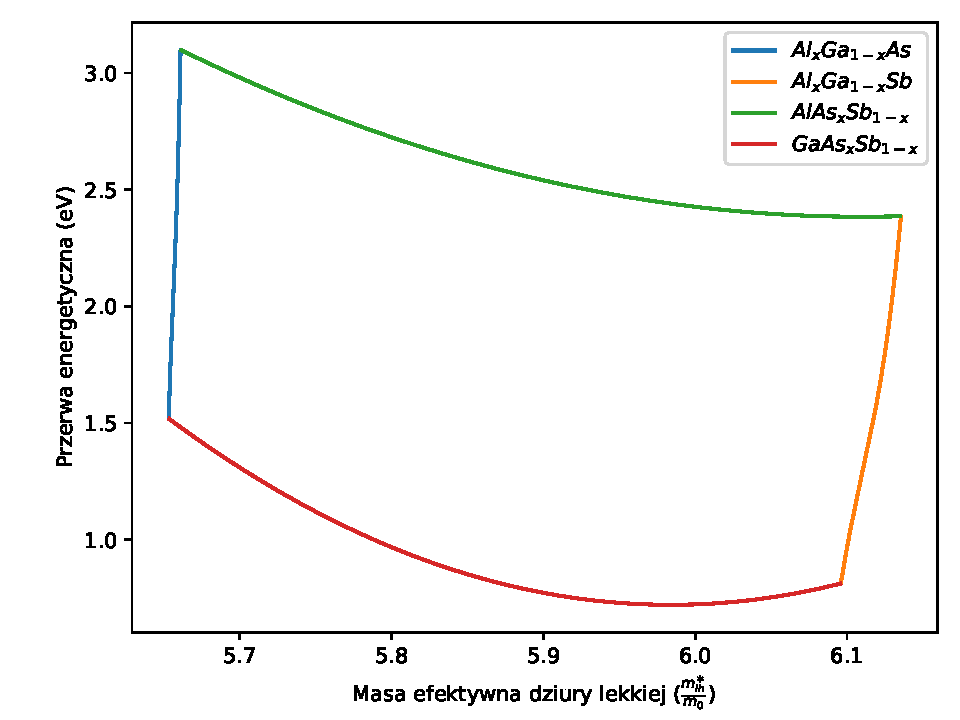
\includegraphics[width = \linewidth]{Figures/ternary/Eg_alc.pdf}
	\caption{Wykres przedstawiający szerokość przerwy wzbronionej w zależności od parametru sieci.
	Zamknięta krzywa stanowi ścieżkę łączącą różne materiały trójskładnikowe.}\label{fig:Eg_alc}
\end{figure}
\pagebreak
Pozostałe wykresy dotyczące parametrów materiałów trójskładnikowych zostały przedstawione w \hyperref[chapt:dodatek]{Dodatku}.\\

Przejdźmy teraz to przedstawienia wyników dla badanego materiału 
czteroskładnikowego tj. \BPChem{Al\_{x}Ga\_{1-x}As\_{y}Sb\_{1-y}}. 
Otrzymano dwie serie wykresów, najpierw dla ustalonego \(x\) w funkcji ułamka
molowego \(y\), a potem dla ustalonego \(y\) w funkcji \(x\). Warto zwrócić uwagę
na przypadki graniczne tj. \(x = 0.0\), \(x =  1.0\) lub \(y = 0.0\), \(y =  1.0\). Wówczas otrzymujemy
krzywe zgodne z wynikami dla stopów trójskładnikowych, przedstawionymi w \hyperref[chapt:dodatek]{Dodatku}.

\subsection{Ustalony \(x\), zmienny \(y\)}
W pierwszej serii wykresów ułamek molowy \(x\) przyjmuje ustalone
wartości wynoszące \([0.0,\;0.2,\; 0.4,\; 0.6,\; 0.8,\; 1.0]\), a ułamek molowy \(y\)
przyjmuje \(1000\) równoodległych wartości między \(0.0\) i \(1.0\).

\begin{itemize}
	\item \(E_g^{\Gamma}\)(eV) --- rysunek~\ref{fig:quat_Eg_x}
	\item VBO (eV) --- rysunek~\ref{fig:quat_vbo_x} 
	\item \(\Delta_{\textrm{SO}}\) --- rysunek~\ref{fig:quat_delta_so_x}
	\item \(a_{lc}\) (\AA) --- rysunek~\ref{fig:quat_alc_x}
	\item \(m_e^{\ast}\) --- rysunek~\ref{fig:quat_me_x}
	\item \(m_{hh}^{\textrm{DOS}}\) --- rysunek~\ref{fig:quat_mhh_x}
	\item \(m_{lh}^{\textrm{DOS}}\) --- rysunek~\ref{fig:quat_mlh_x}
\end{itemize}

\begin{figure}[H]
	\centering
	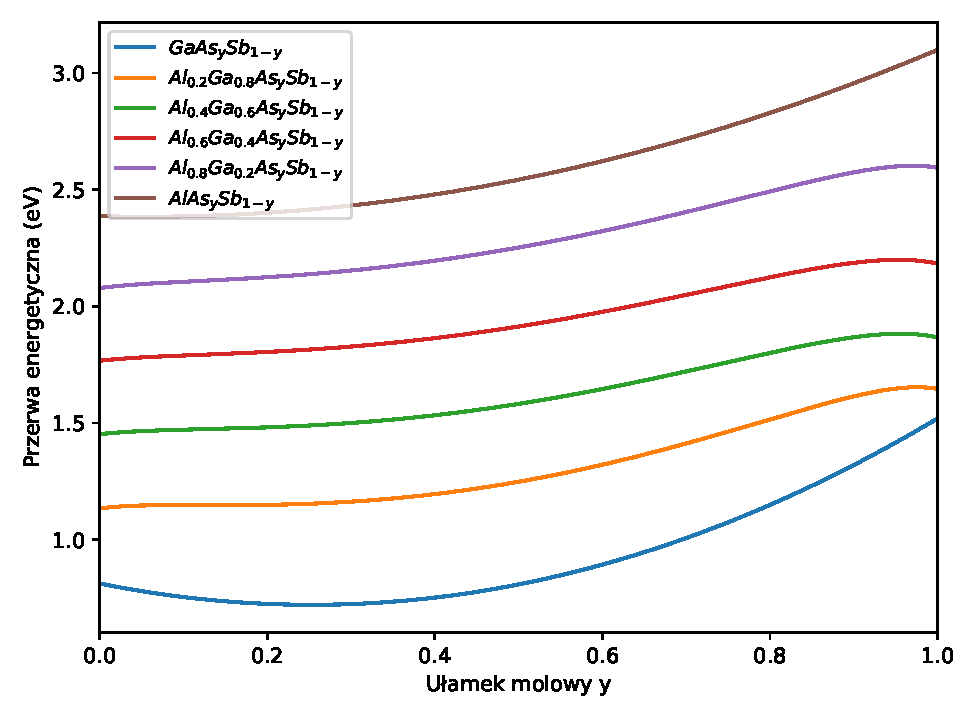
\includegraphics[width = 0.9\linewidth]{Figures/quaternary/quat_eg_x.pdf}
	\caption{Wykres przedstawiający szerokość przerwy wzbronionej w funkcji ułamka 
	molowego.}\label{fig:quat_Eg_x}
\end{figure}

\begin{figure}[H]
	\centering
	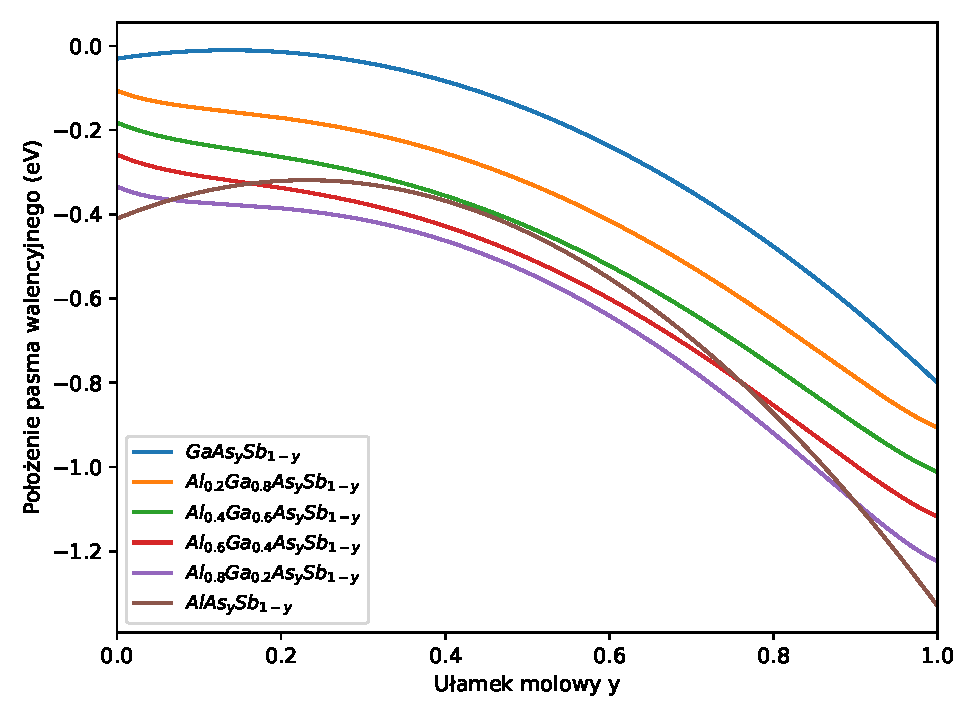
\includegraphics[width = 0.9\linewidth]{Figures/quaternary/quat_vbo_x.pdf}
	\caption{Wykres przedstawiający wierzchołek pasma walencyjnego w funkcji ułamka 
	molowego.}\label{fig:quat_vbo_x}
\end{figure}

\begin{figure}[H]
	\centering
	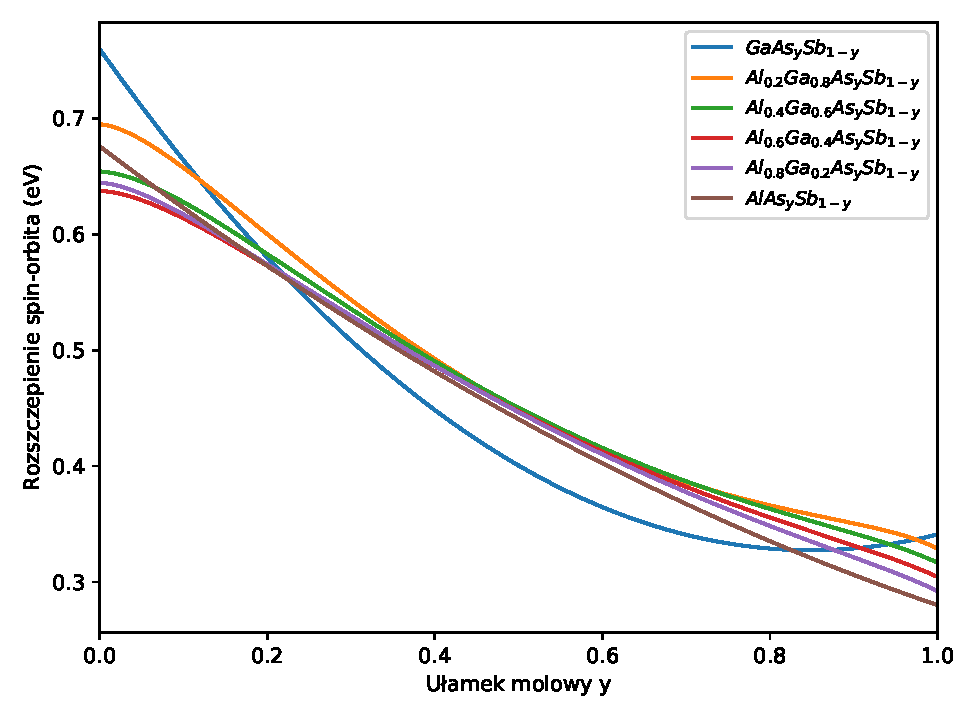
\includegraphics[width = 0.9\linewidth]{Figures/quaternary/quat_delta_so_x.pdf}
	\caption{Wykres przedstawiający rozszczepienie spin-orbita w funkcji ułamka 
	molowego.}\label{fig:quat_delta_so_x}
\end{figure}

\begin{figure}[H]
	\centering
	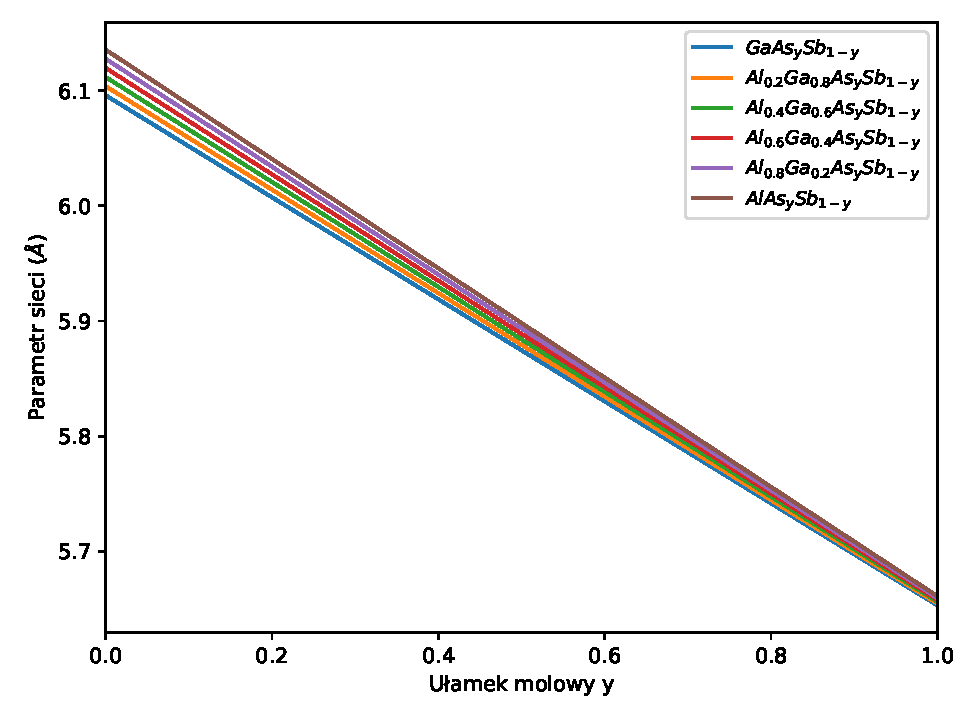
\includegraphics[width = 0.9\linewidth]{Figures/quaternary/quat_alc_x.pdf}
	\caption{Wykres przedstawiający parametr sieciowy w funkcji ułamka 
	molowego.}\label{fig:quat_alc_x}
\end{figure}

\begin{figure}[H]
	\centering
	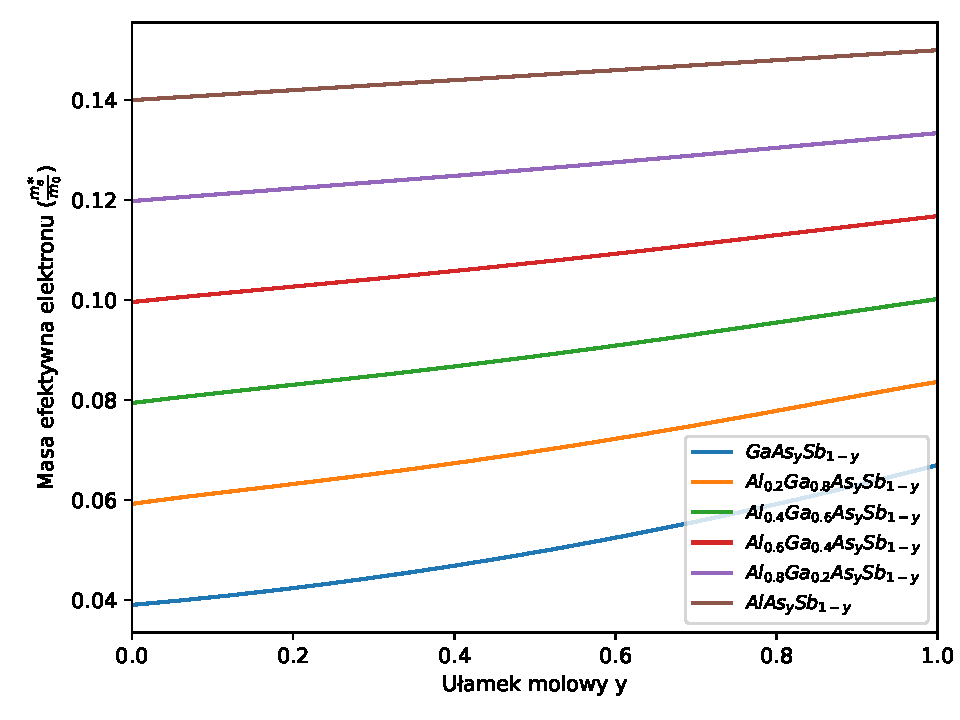
\includegraphics[width = 0.9\linewidth]{Figures/quaternary/quat_m_e_x.pdf}
	\caption{Wykres przedstawiający masę efektywną elektronu w funkcji ułamka 
	molowego.}\label{fig:quat_me_x}
\end{figure}

\begin{figure}[H]
	\centering
	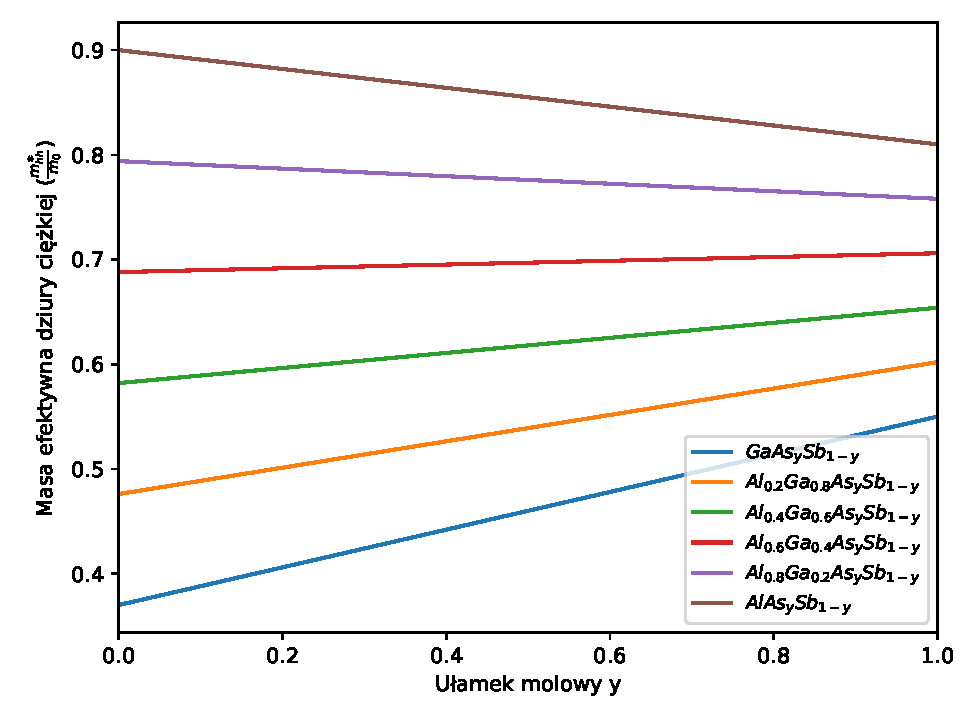
\includegraphics[width = 0.9\linewidth]{Figures/quaternary/quat_m_hh_x.pdf}
	\caption{Wykres przedstawiający masę efektywną ciężkiej dziury w funkcji ułamka 
	molowego.}\label{fig:quat_mhh_x}
\end{figure}

\begin{figure}[H]
	\centering
	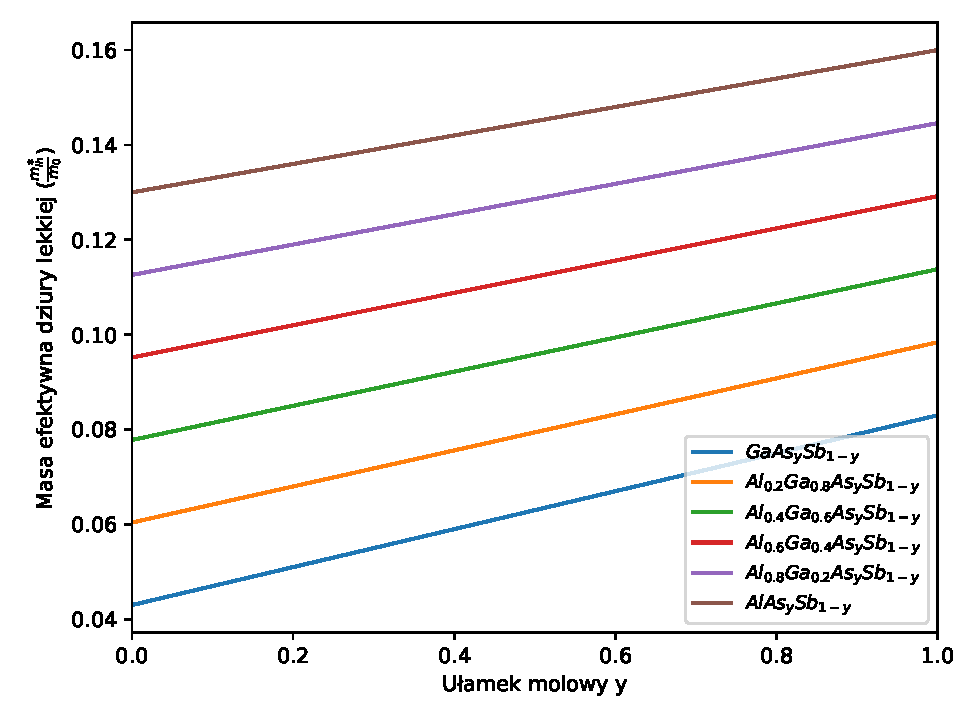
\includegraphics[width = 0.9\linewidth]{Figures/quaternary/quat_m_lh_x.pdf}
	\caption{Wykres przedstawiający masę efektywną lekkiej dziury w funkcji ułamka 
	molowego.}\label{fig:quat_mlh_x}
\end{figure}

\subsection{Ustalony \(y\), zmienny \(x\)}
W drugiej serii wykresów ułamek molowy \(y\) przyjmuje ustalone
wartości wynoszące \([0.0,\;0.2,\; 0.4,\; 0.6,\; 0.8,\; 1.0]\), a ułamek molowy \(x\)
przyjmuje \(1000\) równoodległych wartości między \(0.0\) i \(1.0\). 

\begin{itemize}
	\item \(E_g^{\Gamma}\)(eV) --- rysunek~\ref{fig:quat_Eg_y}
	\item VBO (eV) --- rysunek~\ref{fig:quat_vbo_y} 
	\item \(\Delta_{\textrm{SO}}\) --- rysunek~\ref{fig:quat_delta_so_y}
	\item \(a_{lc}\) (\AA) --- rysunek~\ref{fig:quat_alc_y}
	\item \(m_e^{\ast}\) --- rysunek~\ref{fig:quat_me_y}
	\item \(m_{hh}^{\textrm{DOS}}\) --- rysunek~\ref{fig:quat_mhh_y}
	\item \(m_{lh}^{\textrm{DOS}}\) --- rysunek~\ref{fig:quat_mlh_y}
\end{itemize}
\begin{figure}[H]
	\centering
	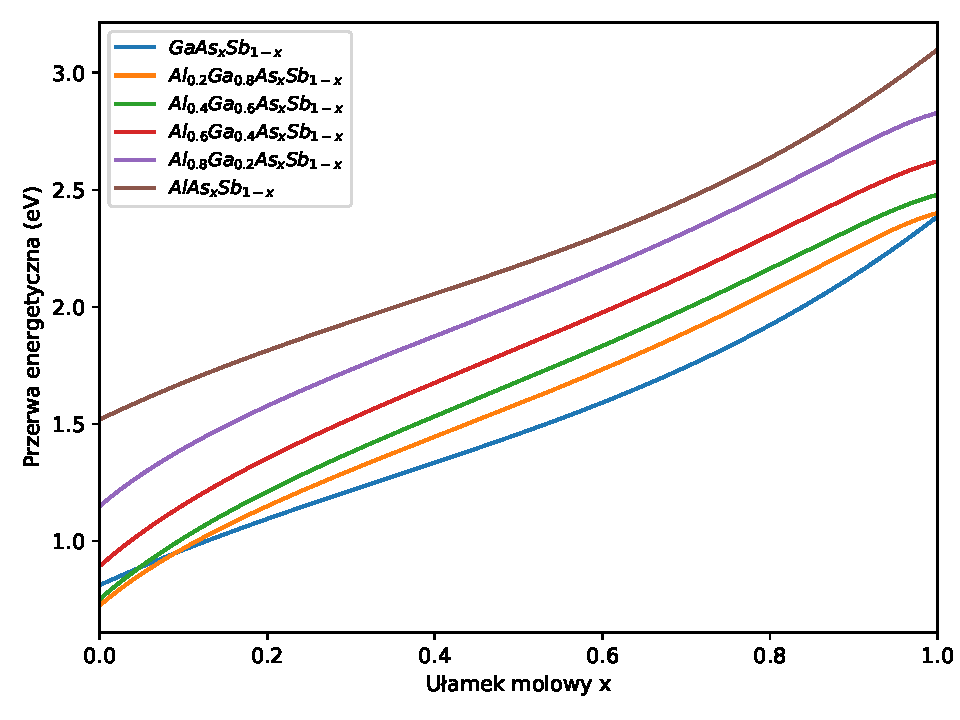
\includegraphics[width = 0.9\linewidth]{Figures/quaternary/quat_eg_y.pdf}
	\caption{Wykres przedstawiający szerokość przerwy wzbronionej w funkcji ułamka 
	molowego.}\label{fig:quat_Eg_y}
\end{figure}

\begin{figure}[H]
	\centering
	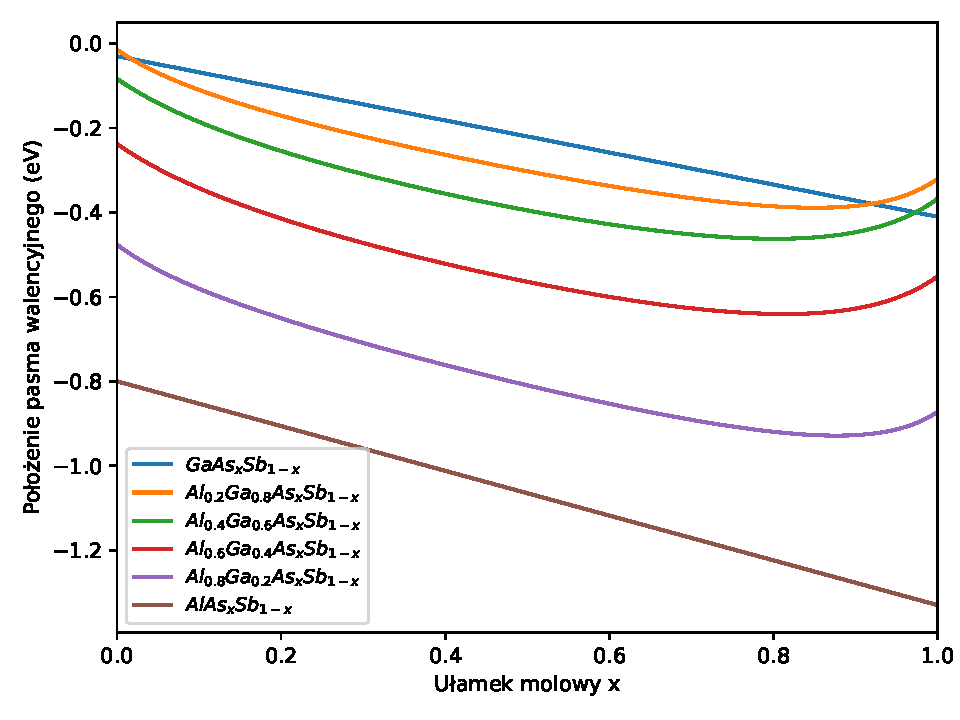
\includegraphics[width = 0.9\linewidth]{Figures/quaternary/quat_vbo_y.pdf}
	\caption{Wykres przedstawiający wierzchołek pasma walencyjnego w funkcji ułamka 
	molowego.}\label{fig:quat_vbo_y}
\end{figure}

\begin{figure}[H]
	\centering
	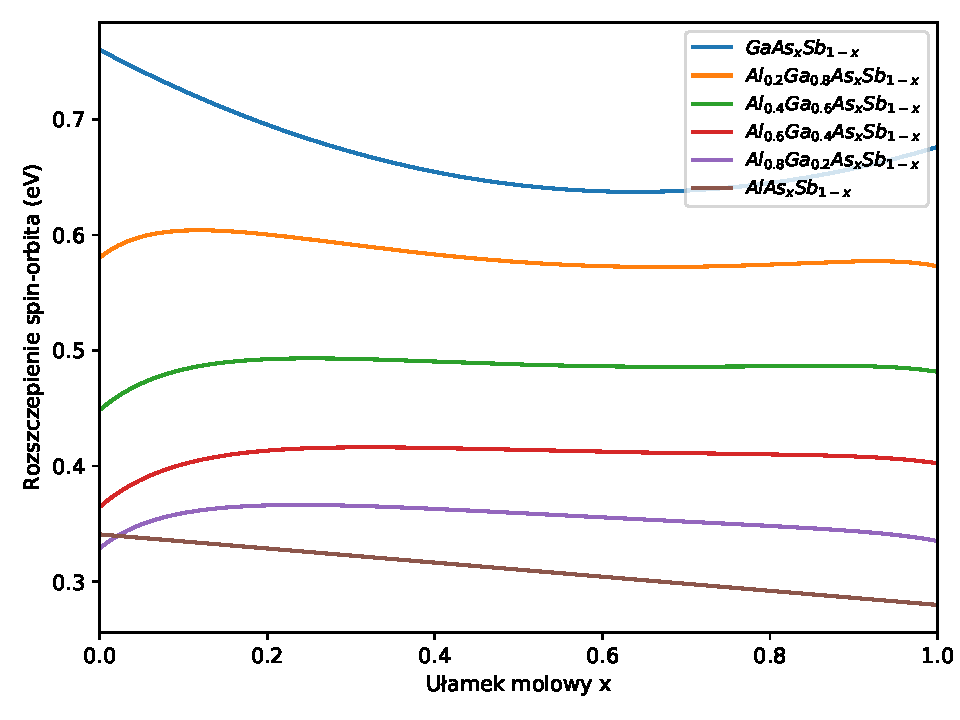
\includegraphics[width = 0.9\linewidth]{Figures/quaternary/quat_delta_so_y.pdf}
	\caption{Wykres przedstawiający rozszczepienie spin-orbita w funkcji ułamka 
	molowego.}\label{fig:quat_delta_so_y}
\end{figure}

\begin{figure}[H]
	\centering
	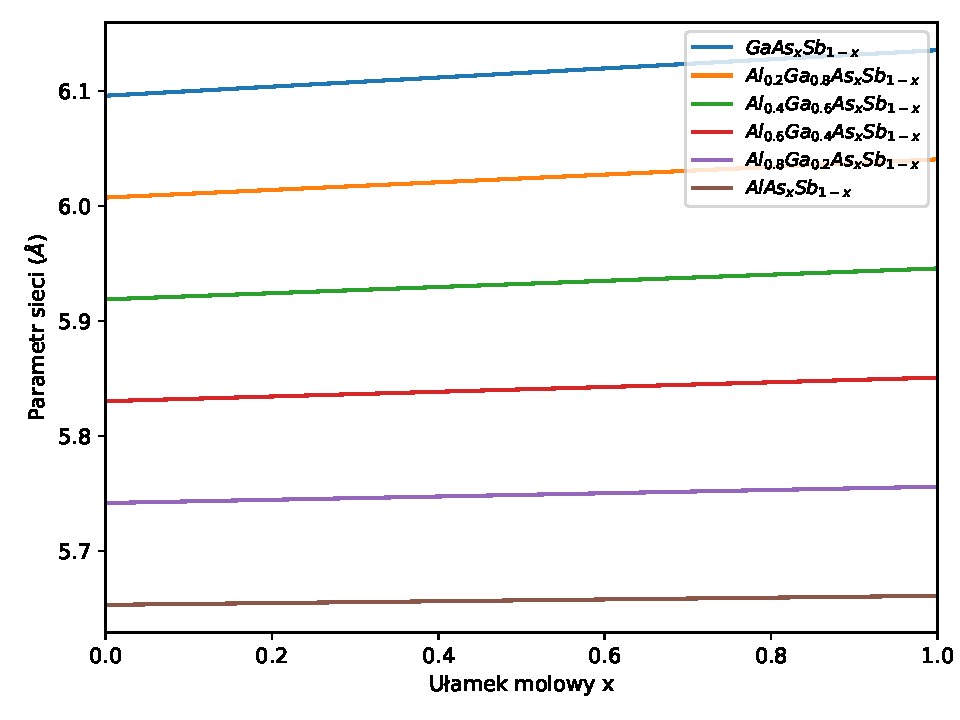
\includegraphics[width = 0.9\linewidth]{Figures/quaternary/quat_alc_y.pdf}
	\caption{Wykres przedstawiający parametr sieciowy w funkcji ułamka 
	molowego.}\label{fig:quat_alc_y}
\end{figure}

\begin{figure}[H]
	\centering
	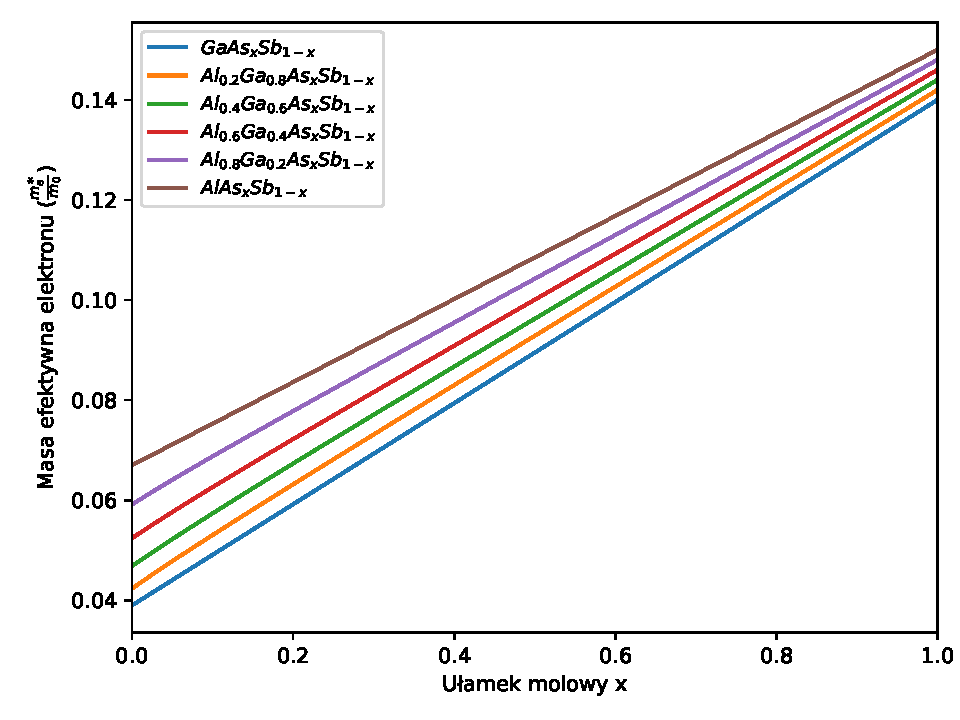
\includegraphics[width = 0.9\linewidth]{Figures/quaternary/quat_m_e_y.pdf}
	\caption{Wykres przedstawiający masę efektywną elektronu w funkcji ułamka 
	molowego.}\label{fig:quat_me_y}
\end{figure}

\begin{figure}[H]
	\centering
	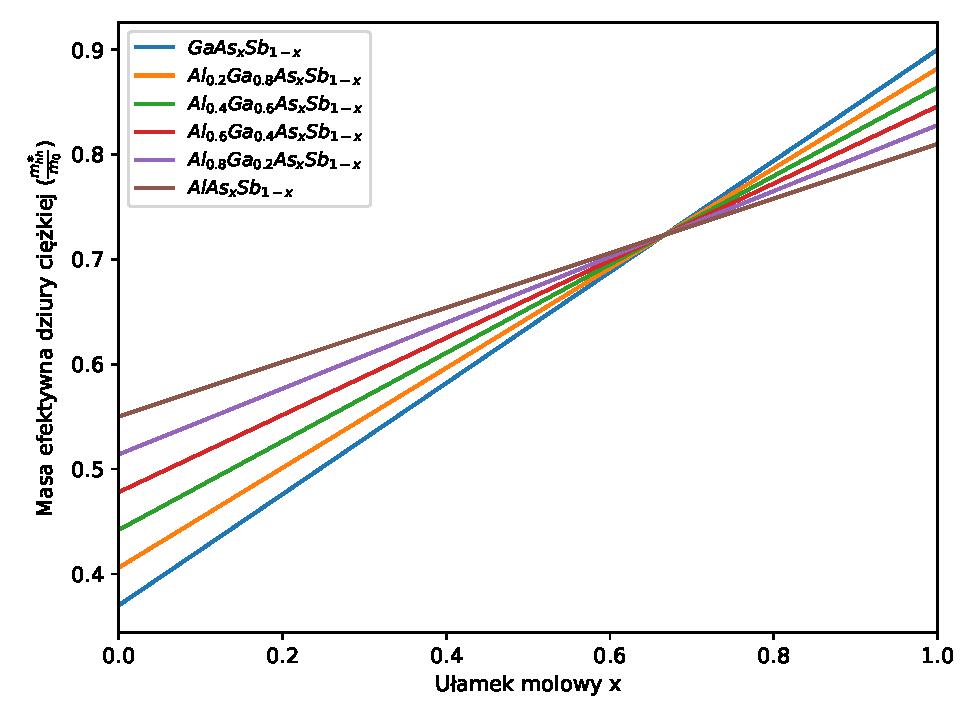
\includegraphics[width = 0.9\linewidth]{Figures/quaternary/quat_m_hh_y.pdf}
	\caption{Wykres przedstawiający masę efektywną ciężkiej dziury w funkcji ułamka 
	molowego.}\label{fig:quat_mhh_y}
\end{figure}

\begin{figure}[H]
	\centering
	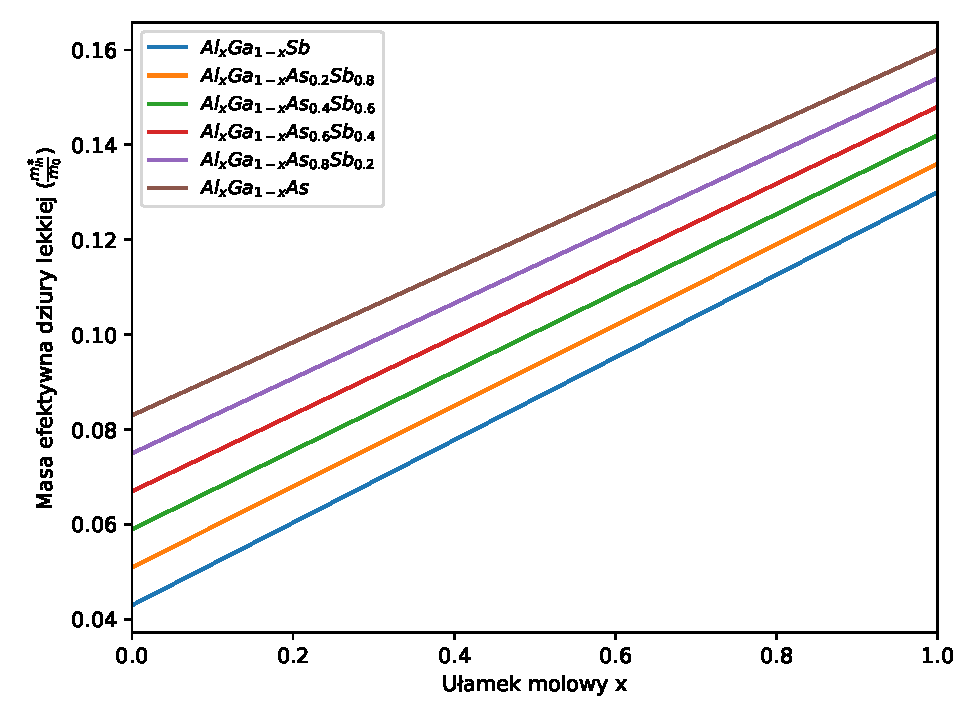
\includegraphics[width = 0.9\linewidth]{Figures/quaternary/quat_m_lh_y.pdf}
	\caption{Wykres przedstawiający masę efektywną lekkiej dziury w funkcji ułamka 
	molowego.}\label{fig:quat_mlh_y}
\end{figure}



\chapter{Wyniki i dyskusja}\label{chapt:results}


\chapter*{Dodatek: Wykresy parametrów materiałów trójskładnikowych}\label{chapt:dodatek}
\addcontentsline{toc}{chapter}{Dodatek: Wykresy parametrów materiałów trójskładnikowych}
Poniżej zostały przestawione wykresy interesujących nas parametrów:
\begin{itemize}
	\item \(E_g^{\Gamma}\)(eV) --- rysunek~\ref{fig:ter_Eg}
	\item VBO (eV) --- rysunek~\ref{fig:ter_vbo} 
	\item \(\Delta_{\textrm{SO}}\) --- rysunek~\ref{fig:ter_delta_so}
	\item \(a_{lc}\) (\AA) --- rysunek~\ref{fig:ter_alc}
	\item \(m_e^{\ast}\) --- rysunek~\ref{fig:ter_me}
	\item \(m_{hh}^{\textrm{DOS}}\) --- rysunek~\ref{fig:ter_mhh}
	\item \(m_{lh}^{\textrm{DOS}}\) --- rysunek~\ref{fig:ter_mlh}
\end{itemize}
\begin{figure}[H]
	\centering
	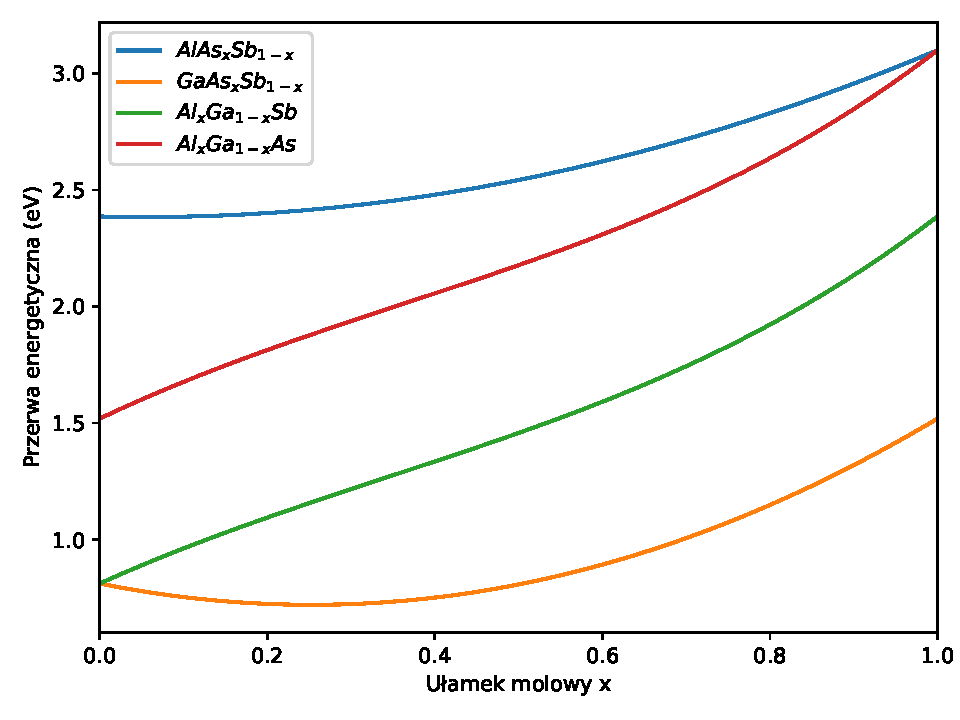
\includegraphics[width = 0.9\linewidth]{Figures/ternary/eg.pdf}
	\caption{Wykres przedstawiający szerokość przerwy wzbronionej w funkcji ułamka 
	molowego.}\label{fig:ter_Eg}
\end{figure}

\begin{figure}[H]
	\centering
	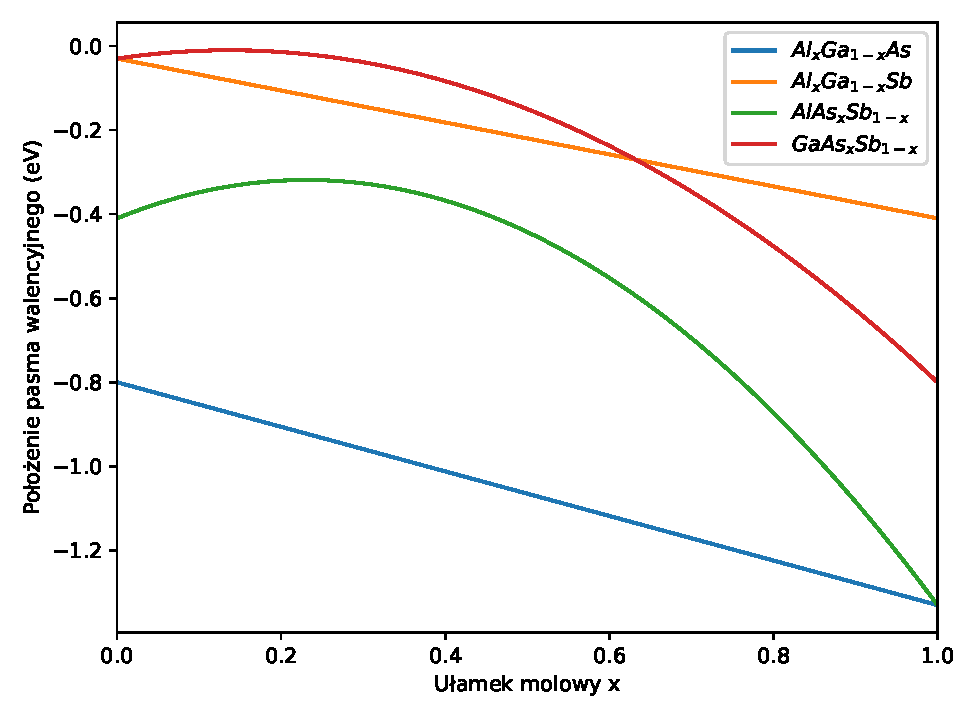
\includegraphics[width = 0.9\linewidth]{Figures/ternary/vbo.pdf}
	\caption{Wykres przedstawiający wierzchołek pasma walencyjnego w funkcji ułamka 
	molowego.}\label{fig:ter_vbo}
\end{figure}

\begin{figure}[H]
	\centering
	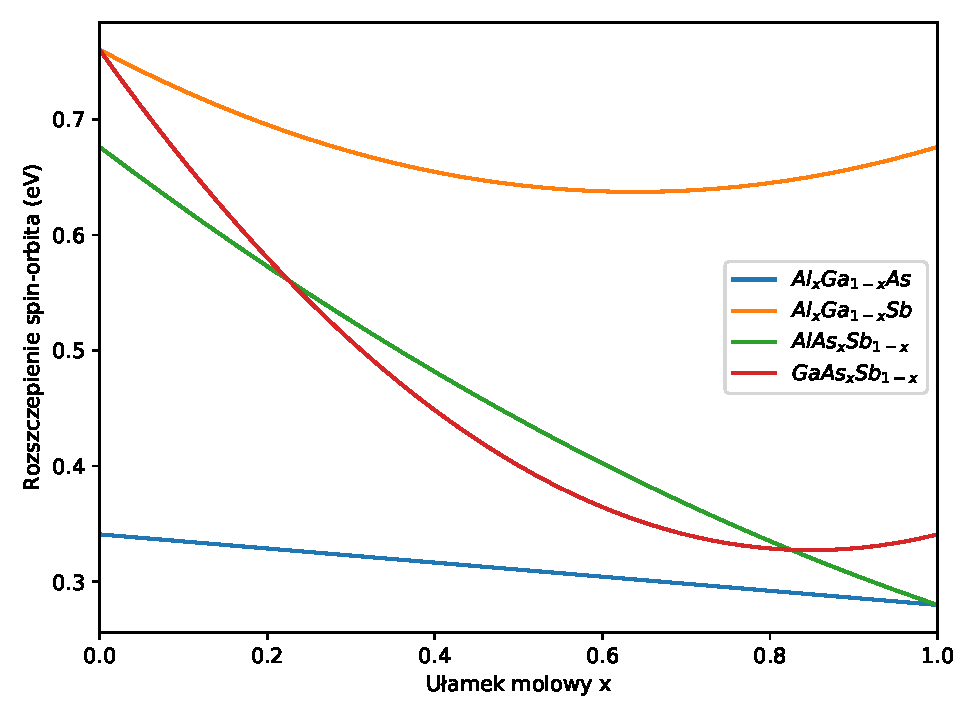
\includegraphics[width = 0.9\linewidth]{Figures/ternary/delta_so.pdf}
	\caption{Wykres przedstawiający rozszczepienie spin-orbita w funkcji ułamka 
	molowego.}\label{fig:ter_delta_so}
\end{figure}

\begin{figure}[H]
	\centering
	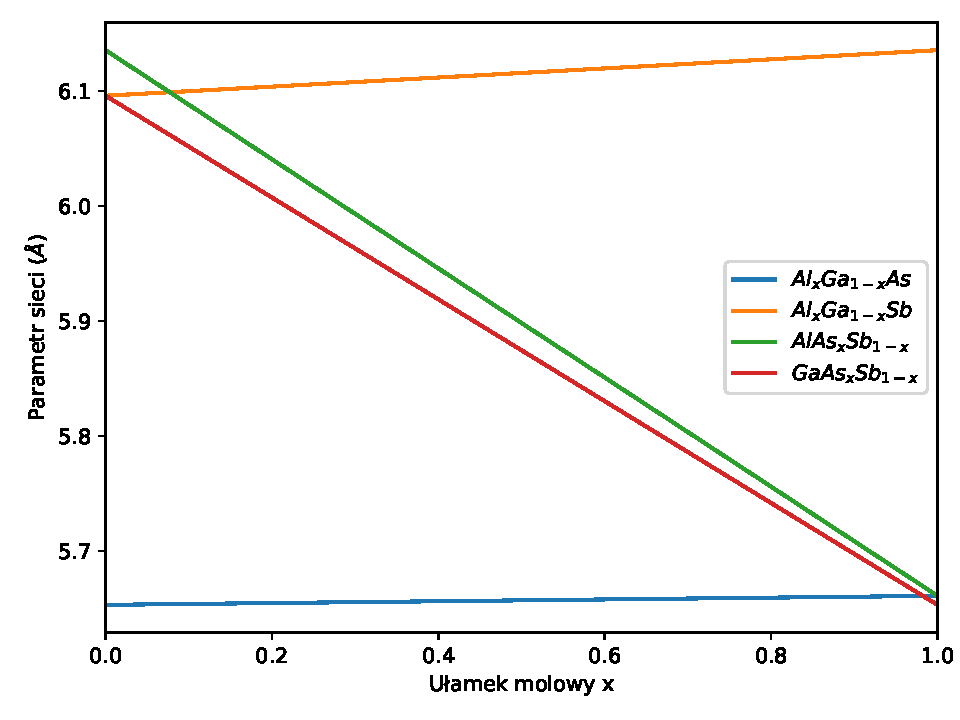
\includegraphics[width = 0.9\linewidth]{Figures/ternary/alc.pdf}
	\caption{Wykres przedstawiający parametr sieciowy w funkcji ułamka 
	molowego.}\label{fig:ter_alc}
\end{figure}

\begin{figure}[H]
	\centering
	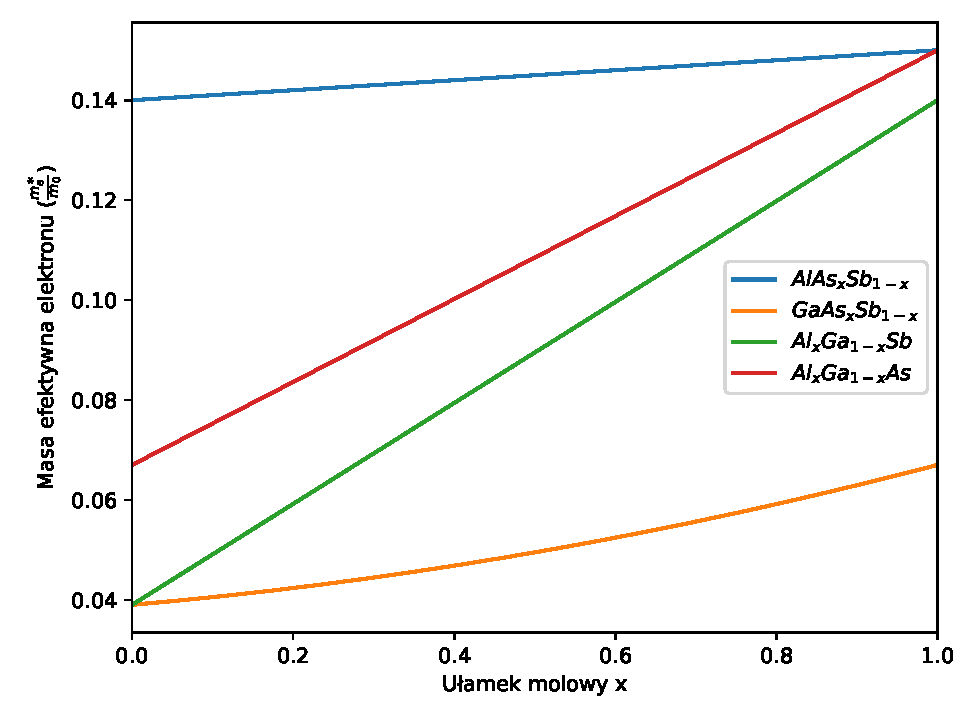
\includegraphics[width = 0.9\linewidth]{Figures/ternary/m_e.pdf}
	\caption{Wykres przedstawiający masę efektywną elektronu w funkcji ułamka 
	molowego.}\label{fig:ter_me}
\end{figure}

\begin{figure}[H]
	\centering
	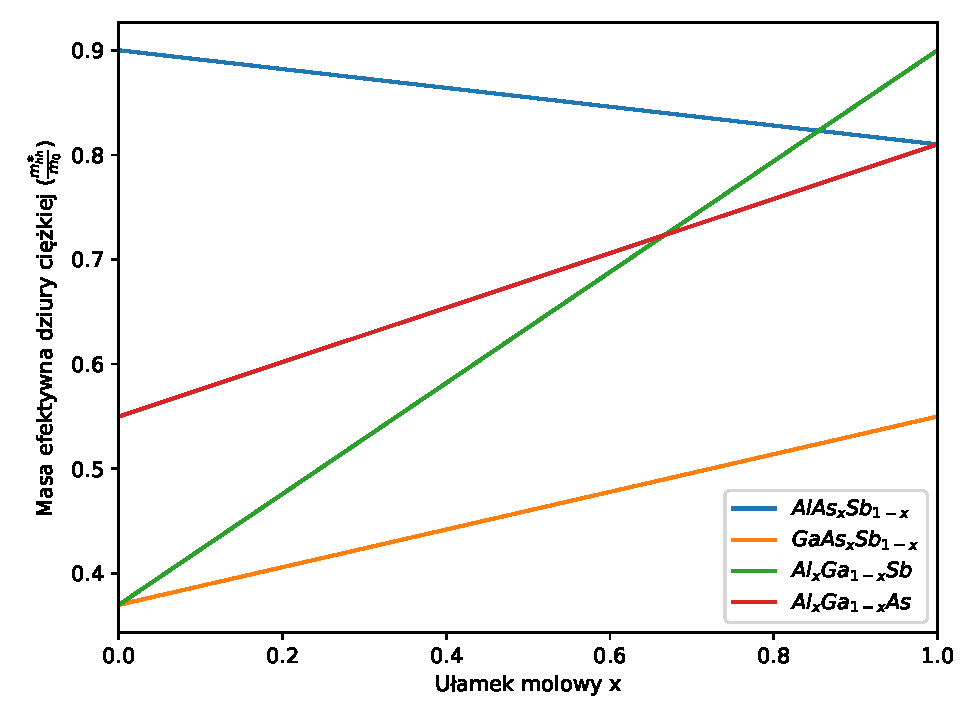
\includegraphics[width = 0.9\linewidth]{Figures/ternary/m_hh.pdf}
	\caption{Wykres przedstawiający masę efektywną ciężkiej dziury w funkcji ułamka 
	molowego.}\label{fig:ter_mhh}
\end{figure}

\begin{figure}[H]
	\centering
	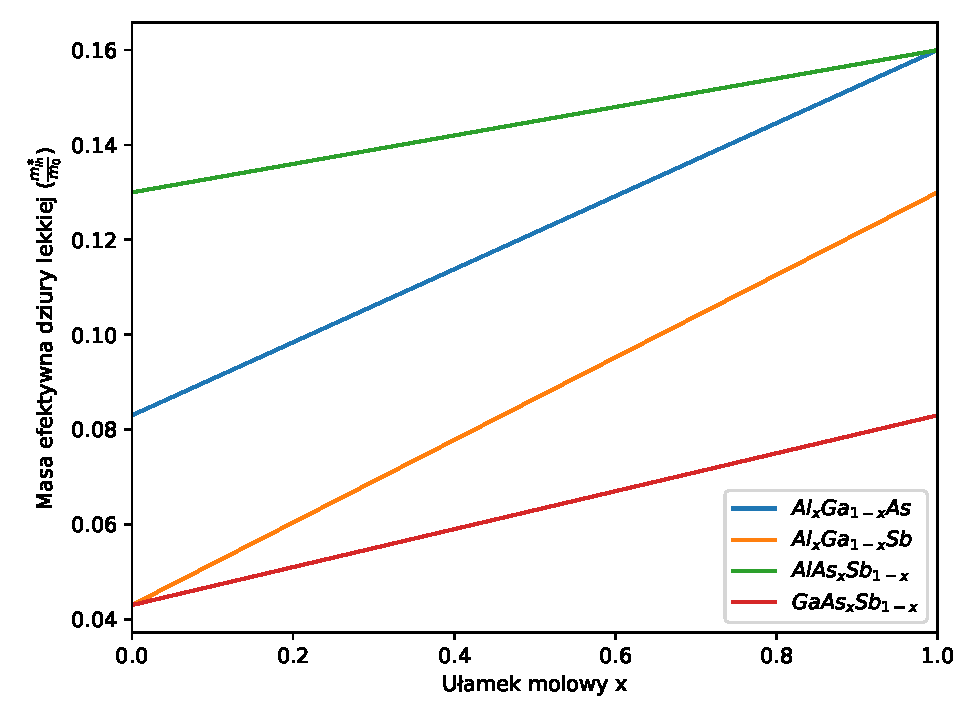
\includegraphics[width = 0.9\linewidth]{Figures/ternary/m_lh.pdf}
	\caption{Wykres przedstawiający masę efektywną lekkiej dziury w funkcji ułamka 
	molowego.}\label{fig:ter_mlh}
\end{figure}


	

	
	% Adding a bibliography if citations are used in the report
	% Un/Comment the following line to customize the Bibliography title
	\renewcommand{\bibname}{Bibliografia}
	
	% \bibliography{AlGaAsSb.bib}
	
	% Uncomment the following two lines to remvoe the cc license
	% \vspace*{\fill}
	% {\hypersetup{urlcolor=black}{\scriptsize \doclicenseThis}}
	% Adds reference to the Bibliography in the ToC
	\addcontentsline{toc}{chapter}{\bibname}
	\printbibliography{}
	 \pagebreak
	
	
		

\end{document}